% Created 2021-03-08 man 17:34
% Intended LaTeX compiler: pdflatex
\documentclass[12pt]{article}

%%%% settings when exporting code %%%% 

\usepackage{listings}
\lstdefinestyle{code-small}{
backgroundcolor=\color{white}, % background color for the code block
basicstyle=\ttfamily\small, % font used to display the code
commentstyle=\color[rgb]{0.5,0,0.5}, % color used to display comments in the code
keywordstyle=\color{black}, % color used to highlight certain words in the code
numberstyle=\ttfamily\tiny\color{gray}, % color used to display the line numbers
rulecolor=\color{black}, % color of the frame
stringstyle=\color[rgb]{0,.5,0},  % color used to display strings in the code
breakatwhitespace=false, % sets if automatic breaks should only happen at whitespace
breaklines=true, % sets automatic line breaking
columns=fullflexible,
frame=single, % adds a frame around the code (non,leftline,topline,bottomline,lines,single,shadowbox)
keepspaces=true, % % keeps spaces in text, useful for keeping indentation of code
literate={~}{$\sim$}{1}, % symbol properly display via latex
numbers=none, % where to put the line-numbers; possible values are (none, left, right)
numbersep=10pt, % how far the line-numbers are from the code
showspaces=false,
showstringspaces=false,
stepnumber=1, % the step between two line-numbers. If it's 1, each line will be numbered
tabsize=1,
xleftmargin=0cm,
emph={anova,apply,class,coef,colnames,colNames,colSums,dim,dcast,for,ggplot,head,if,ifelse,is.na,lapply,list.files,library,logLik,melt,plot,require,rowSums,sapply,setcolorder,setkey,str,summary,tapply},
aboveskip = \medskipamount, % define the space above displayed listings.
belowskip = \medskipamount, % define the space above displayed listings.
lineskip = 0pt} % specifies additional space between lines in listings
\lstset{style=code-small}
%%%% packages %%%%%

\usepackage[utf8]{inputenc}
\usepackage[T1]{fontenc}
\usepackage{lmodern}
\usepackage{textcomp}
\usepackage{color}
\usepackage{graphicx}
\usepackage{grffile}
\usepackage{wrapfig}
\usepackage{rotating}
\usepackage{longtable}
\usepackage{multirow}
\usepackage{multicol}
\usepackage{changes}
\usepackage{pdflscape}
\usepackage{geometry}
\usepackage[normalem]{ulem}
\usepackage{amssymb}
\usepackage{amsmath}
\usepackage{amsfonts}
\usepackage{dsfont}
\usepackage{array}
\usepackage{ifthen}
\usepackage{hyperref}
\usepackage{natbib}
\RequirePackage{setspace} % to modify the space between lines - incompatible with footnote in beamer
\renewcommand{\baselinestretch}{1.1}
\geometry{top=1cm}
\usepackage{titlesec}
\usepackage{etoolbox}
\makeatletter
\patchcmd{\ttlh@hang}{\parindent\z@}{\parindent\z@\leavevmode}{}{}
\patchcmd{\ttlh@hang}{\noindent}{}{}{}
\makeatother
\RequirePackage{colortbl} % arrayrulecolor to mix colors
\definecolor{myorange}{rgb}{1,0.2,0}
\definecolor{mypurple}{rgb}{0.7,0,8}
\definecolor{mycyan}{rgb}{0,0.6,0.6}
\newcommand{\lightblue}{blue!50!white}
\newcommand{\darkblue}{blue!80!black}
\newcommand{\darkgreen}{green!50!black}
\newcommand{\darkred}{red!50!black}
\definecolor{gray}{gray}{0.5}
\hypersetup{
citecolor=[rgb]{0,0.5,0},
urlcolor=[rgb]{0,0,0.5},
linkcolor=[rgb]{0,0,0.5},
}
\newenvironment{comment}{\small \color{gray}\fontfamily{lmtt}\selectfont}{\par}
\newenvironment{activity}{\color{orange}\fontfamily{qzc}\selectfont}{\par}
\RequirePackage{pifont}
\RequirePackage{relsize}
\newcommand{\Cross}{{\raisebox{-0.5ex}%
{\relsize{1.5}\ding{56}}}\hspace{1pt} }
\newcommand{\Valid}{{\raisebox{-0.5ex}%
{\relsize{1.5}\ding{52}}}\hspace{1pt} }
\newcommand{\CrossR}{ \textcolor{red}{\Cross} }
\newcommand{\ValidV}{ \textcolor{green}{\Valid} }
\usepackage{stackengine}
\usepackage{scalerel}
\newcommand\Warning[1][3ex]{%
\renewcommand\stacktype{L}%
\scaleto{\stackon[1.3pt]{\color{red}$\triangle$}{\tiny\bfseries !}}{#1}%
\xspace
}
\newcommand\Rlogo{\textbf{\textsf{R}}\xspace} %
\RequirePackage{fancyvrb}
\DefineVerbatimEnvironment{verbatim}{Verbatim}{fontsize=\small,formatcom = {\color[rgb]{0.5,0,0}}}
\lstdefinestyle{code-tiny}{basicstyle=\ttfamily\footnotesize}
\RequirePackage{enumitem} % better than enumerate
\RequirePackage{epstopdf} % to be able to convert .eps to .pdf image files
\RequirePackage{capt-of} %
\RequirePackage{caption} % newlines in graphics
\RequirePackage{tikz-cd} % graph
\RequirePackage{booktabs} % for nice lines in table (e.g. toprule, bottomrule, midrule, cmidrule)
\RequirePackage{amsmath}
\RequirePackage{algorithm}
\RequirePackage[noend]{algpseudocode}
\RequirePackage{dsfont}
\RequirePackage{amsmath,stmaryrd,graphicx}
\RequirePackage{prodint} % product integral symbol (\PRODI)
\usepackage{ifthen}
\usepackage{xifthen}
\usepackage{xargs}
\usepackage{xspace}
\newcommand\defOperator[7]{%
\ifthenelse{\isempty{#2}}{
\ifthenelse{\isempty{#1}}{#7{#3}#4}{#7{#3}#4 \left#5 #1 \right#6}
}{
\ifthenelse{\isempty{#1}}{#7{#3}#4_{#2}}{#7{#3}#4_{#1}\left#5 #2 \right#6}
}
}
\newcommand\defUOperator[5]{%
\ifthenelse{\isempty{#1}}{
#5\left#3 #2 \right#4
}{
\ifthenelse{\isempty{#2}}{\underset{#1}{\operatornamewithlimits{#5}}}{
\underset{#1}{\operatornamewithlimits{#5}}\left#3 #2 \right#4}
}
}
\newcommand{\defBoldVar}[2]{
\ifthenelse{\equal{#2}{T}}{\boldsymbol{#1}}{\mathbf{#1}}
}
\newcommandx\Esp[2][1=,2=]{\defOperator{#1}{#2}{E}{}{\lbrack}{\rbrack}{\mathbb}}
\newcommandx\Prob[2][1=,2=]{\defOperator{#1}{#2}{P}{}{\lbrack}{\rbrack}{\mathbb}}
\newcommandx\Qrob[2][1=,2=]{\defOperator{#1}{#2}{Q}{}{\lbrack}{\rbrack}{\mathbb}}
\newcommandx\Var[2][1=,2=]{\defOperator{#1}{#2}{V}{ar}{\lbrack}{\rbrack}{\mathbb}}
\newcommandx\Cov[2][1=,2=]{\defOperator{#1}{#2}{C}{ov}{\lbrack}{\rbrack}{\mathbb}}
\newcommandx\Binom[2][1=,2=]{\defOperator{#1}{#2}{B}{}{(}{)}{\mathcal}}
\newcommandx\Gaus[2][1=,2=]{\defOperator{#1}{#2}{N}{}{(}{)}{\mathcal}}
\newcommandx\Wishart[2][1=,2=]{\defOperator{#1}{#2}{W}{ishart}{(}{)}{\mathcal}}
\newcommandx\Likelihood[2][1=,2=]{\defOperator{#1}{#2}{L}{}{(}{)}{\mathcal}}
\newcommandx\logLikelihood[2][1=,2=]{\defOperator{#1}{#2}{\ell}{}{(}{)}{}}
\newcommandx\Information[2][1=,2=]{\defOperator{#1}{#2}{I}{}{(}{)}{\mathcal}}
\newcommandx\Score[2][1=,2=]{\defOperator{#1}{#2}{S}{}{(}{)}{\mathcal}}
\newcommandx\Vois[2][1=,2=]{\defOperator{#1}{#2}{V}{}{(}{)}{\mathcal}}
\newcommandx\IF[2][1=,2=]{\defOperator{#1}{#2}{IF}{}{(}{)}{\mathcal}}
\newcommandx\Ind[1][1=]{\defOperator{}{#1}{1}{}{(}{)}{\mathds}}
\newcommandx\Max[2][1=,2=]{\defUOperator{#1}{#2}{(}{)}{min}}
\newcommandx\Min[2][1=,2=]{\defUOperator{#1}{#2}{(}{)}{max}}
\newcommandx\argMax[2][1=,2=]{\defUOperator{#1}{#2}{(}{)}{argmax}}
\newcommandx\argMin[2][1=,2=]{\defUOperator{#1}{#2}{(}{)}{argmin}}
\newcommandx\cvD[2][1=D,2=n \rightarrow \infty]{\xrightarrow[#2]{#1}}
\newcommandx\Hypothesis[2][1=,2=]{
\ifthenelse{\isempty{#1}}{
\mathcal{H}
}{
\ifthenelse{\isempty{#2}}{
\mathcal{H}_{#1}
}{
\mathcal{H}^{(#2)}_{#1}
}
}
}
\newcommandx\dpartial[4][1=,2=,3=,4=\partial]{
\ifthenelse{\isempty{#3}}{
\frac{#4 #1}{#4 #2}
}{
\left.\frac{#4 #1}{#4 #2}\right\rvert_{#3}
}
}
\newcommandx\dTpartial[3][1=,2=,3=]{\dpartial[#1][#2][#3][d]}
\newcommandx\ddpartial[3][1=,2=,3=]{
\ifthenelse{\isempty{#3}}{
\frac{\partial^{2} #1}{\partial #2^2}
}{
\frac{\partial^2 #1}{\partial #2\partial #3}
}
}
\newcommand\Real{\mathbb{R}}
\newcommand\Rational{\mathbb{Q}}
\newcommand\Natural{\mathbb{N}}
\newcommand\trans[1]{{#1}^\intercal}%\newcommand\trans[1]{{\vphantom{#1}}^\top{#1}}
\newcommand{\independent}{\mathrel{\text{\scalebox{1.5}{$\perp\mkern-10mu\perp$}}}}
\newcommand\half{\frac{1}{2}}
\newcommand\normMax[1]{\left|\left|#1\right|\right|_{max}}
\newcommand\normTwo[1]{\left|\left|#1\right|\right|_{2}}
\newcommand\Veta{\boldsymbol{\eta}}
\newcommand\VX{\mathbf{X}}
\author{Brice Ozenne}
\date{\today}
\title{Latent variable model and identifiability}
\hypersetup{
 colorlinks=true,
 pdfauthor={Brice Ozenne},
 pdftitle={Latent variable model and identifiability},
 pdfkeywords={},
 pdfsubject={},
 pdfcreator={Emacs 27.0.50 (Org mode 9.0.4)},
 pdflang={English}
 }
\begin{document}

\maketitle
\lstset{style=code-tiny}

\section{A necessary condition for identifiability}
\label{sec:orgc137cef}
One way to assess identifiability of a model is to count the number of
parameters vs. the number of sufficient statistics brought by the
data. If the number of parameters in the model exceed the number of
sufficient statistics brought by the data the model is not
identifiable.

\subsection{Example in univariate linear models}
\label{sec:org19d7c4f}
Assuming normaly distributed variables:

\bigskip

\lstset{language=r,label= ,caption= ,captionpos=b,numbers=none}
\begin{lstlisting}
set.seed(10)
data <- data.frame(Y = rnorm(10),
		   X = rnorm(10))
\end{lstlisting}

\bigskip

the sufficient statistics are the mean, variance, and covariance. This
means that knowing the mean and the variance, I can simulate new data
following the same law as my observed data. When considering only the
outcome, I need at least two observations to fit a linear model:

\bigskip

\lstset{language=r,label= ,caption= ,captionpos=b,numbers=none}
\begin{lstlisting}
## can only estimate the mean of Y
eY.1 <- lm(Y ~ 1, data = data[1,, drop = FALSE])
summary(eY.1)$coef
sigma(eY.1)
\end{lstlisting}

\begin{verbatim}
              Estimate Std. Error t value Pr(>|t|)
(Intercept) 0.01874617        NaN     NaN      NaN
[1] NaN
\end{verbatim}

\clearpage

\lstset{language=r,label= ,caption= ,captionpos=b,numbers=none}
\begin{lstlisting}
## can estimate both the mean and variance of Y
eY.2 <- lm(Y ~ 1, data = data[1:2,, drop = FALSE])
summary(eY.2)$coef
sigma(eY.2)
\end{lstlisting}

\begin{verbatim}
               Estimate Std. Error    t value  Pr(>|t|)
(Intercept) -0.08275319  0.1014994 -0.8153075 0.5645487
[1] 0.1435418
\end{verbatim}


\bigskip

If I also want to adjust on X, I now also need to estimate the
covariance between X and Y. So I need at least one more observation:

\bigskip

\lstset{language=r,label= ,caption= ,captionpos=b,numbers=none}
\begin{lstlisting}
## can only estimate the mean of Y and its covariance with X
eXY.2 <- lm(Y ~ X, data = data[1:2,, drop = FALSE])
summary(eXY.2)$coef
sigma(eXY.2)
\end{lstlisting}

\begin{verbatim}
              Estimate Std. Error t value Pr(>|t|)
(Intercept) -0.6276732        NaN     NaN      NaN
X            0.5867049        NaN     NaN      NaN
[1] NaN
\end{verbatim}

\lstset{language=r,label= ,caption= ,captionpos=b,numbers=none}
\begin{lstlisting}
## can estimate the mean, variance of Y and its covariance with X
eXY.3 <- lm(Y ~ X, data = data[1:3,, drop = FALSE])
summary(eXY.3)$coef
sigma(eXY.3)
\end{lstlisting}

\begin{verbatim}
             Estimate Std. Error    t value   Pr(>|t|)
(Intercept) -1.091006 0.09766722 -11.170647 0.05683890
X            1.072162 0.12464616   8.601644 0.07368065
[1] 0.1226233
\end{verbatim}

\clearpage

\section{Application to latent variable models (lvm)}
\label{sec:org969b607}

In a latent variable model things are simular. Because we are interested in modeling the
relationship between variables, usually we focus on the covariance matrix: does the observed
covariance matrix enable to identify the modeled covariance matrix? 

\subsection{Example 1: bivariate lvm}
\label{sec:org6528678}
Consider the following model:

\lstset{language=r,label= ,caption= ,captionpos=b,numbers=none}
\begin{lstlisting}
library(lava)

lvm.2Y <- lvm(c(Y, E) ~ eta)
latent(lvm.2Y) <- ~ eta
\end{lstlisting}

\begin{center}
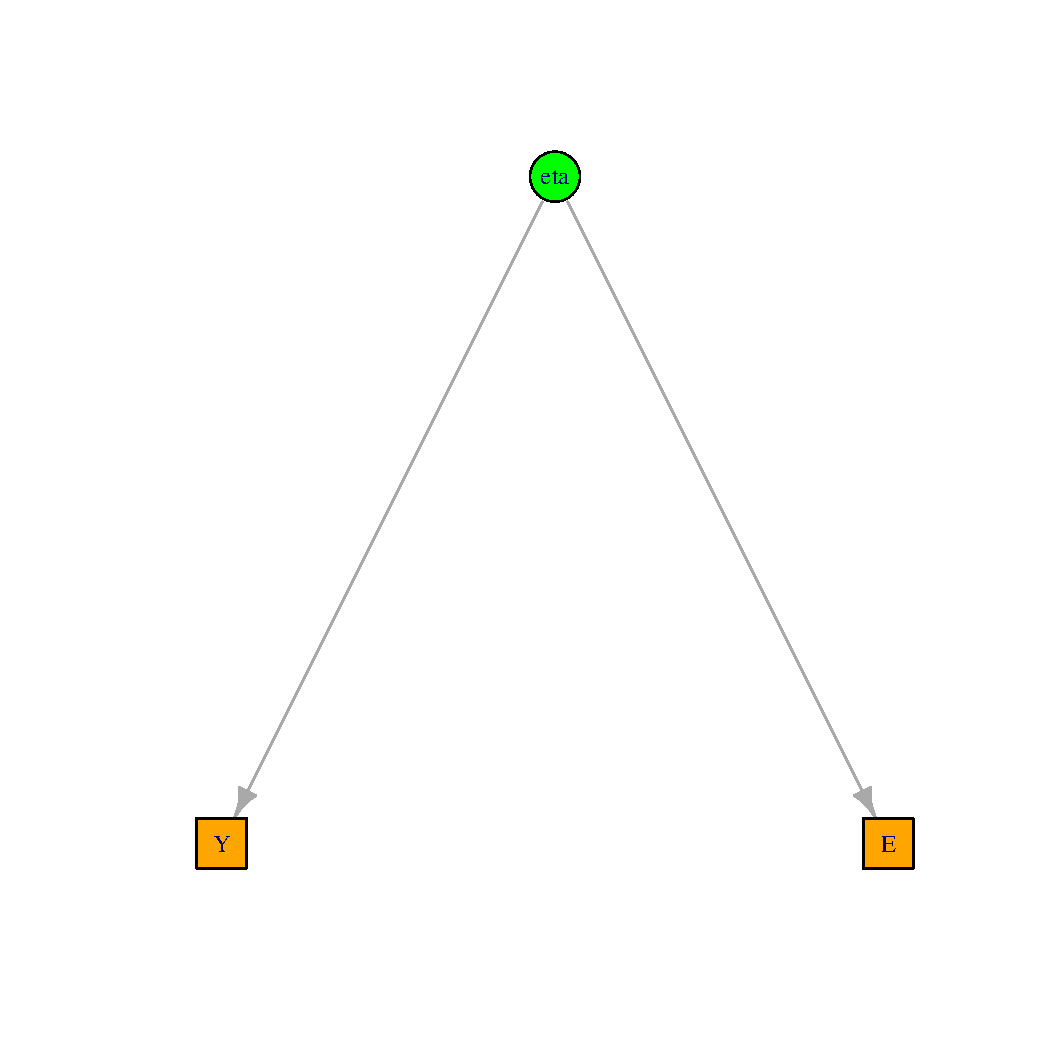
\includegraphics[width=0.5\textwidth]{./figures/show-bivariateLVM.pdf}
\end{center}

This model involves 3 variables (2 observed and 1 latent). We can
write the (full)  \textbf{mean vector} and \textbf{variance-covariance matrix} between all the variables:
\begin{align*}
\mu = \begin{bmatrix} 
\mu_Y \\ \mu_\eta \\ \mu_E \\
\end{bmatrix} = \begin{bmatrix} 
\Esp[Y] \\ \Esp[\eta] \\ \Esp[E] \\
\end{bmatrix} 
\qquad 
\Sigma = \begin{bmatrix} 
\sigma_{Y,Y} & \sigma_{Y,\eta} & \sigma_{Y,E} \\ & \sigma_{\eta,\eta} & \sigma_{\eta,E} \\ & & \sigma_{E,E}  \\
\end{bmatrix} = \begin{bmatrix} 
\Var(Y) & \Cov(Y,\eta) & \Cov(Y,E) \\ & \Var(\eta) & \Cov(\eta,E) \\ & & \Var(E)  \\
\end{bmatrix} 
\end{align*}
Since we don't observed \(\eta\), we cannot estimate its mean and
variance. A common convention is to set its mean to \(0\) and variance
to \(1\) \footnote{By default, \texttt{lava} do something else: it sets the
mean of \(Y\), the reference outcome, to 0 and fix its covariance such
that \(\Cov(Y,\eta)=\Var(\eta)\)}. Using this latent variable model, we
also assumed here that \(Y\) is independent of \(E\) given \(\eta\)
(i.e. \(\Cov(Y,\eta)=\frac{\Cov(Y,\eta)\Cov(E,\eta)}{\Var[\eta]}\)). So
at the end of the day, we only have 4 parameters to estimate: 
\begin{align*}
\theta = \left(\mu_Y,\mu_E, \sigma_{Y,Y}, \sigma_{Y,\eta}, \sigma_{\eta,E}, \sigma_{E,E}\right)
\end{align*}
\clearpage

The \textbf{empirical mean vector} contains two parameters but the \textbf{empirical
variance-covariance matrix} only contains three different parameters:
\begin{align*}
m = 
\begin{bmatrix} 
\overline{Y} \\ \overline{E} \\
\end{bmatrix} 
\qquad
S = 
\begin{bmatrix} 
s_{Y,Y} & s_{Y,E} \\ & s_{E,E} \\
\end{bmatrix} 
\end{align*}

We can check that in R:
\lstset{language=r,label= ,caption= ,captionpos=b,numbers=none}
\begin{lstlisting}
n <- 1e3
df.2Y <- sim(lvm.2Y, n, latent = FALSE)
cbind(mu=colMeans(df.2Y), vcov = cov(df.2Y))
\end{lstlisting}

\begin{verbatim}
           mu         Y         E
Y -0.01663862 2.0403977 0.9651849
E  0.06287055 0.9651849 1.9554924
\end{verbatim}

Overall:
\begin{description}
\item[{\ValidV}] for the mean parameters: the full expectation vector would contain 3
parameters, one for each variable. We only observe two of them
(\(Y\) and \(E\)) and by default lava fix the intercept of \(Y\) to
be 0 so there are only two mean parameters.
\item[{\CrossR}] for the variance-covariance parameters: we have 6
parameters to estimate (3 variances, 3 covariances) which
after applying some necessary restriction reduces to 4
parameters. However we only observe 3 moments. The model
is therefore not identifiable.
\end{description}
This means that the lvm won't properly converge
\lstset{language=r,label= ,caption= ,captionpos=b,numbers=none}
\begin{lstlisting}
estimate(lvm(Y ~ eta, E ~ eta, eta[0:1] ~ 1), 
	 data = df.2Y)
\end{lstlisting}

\begin{verbatim}
                    Estimate Std. Error  Z-value  P-value
Measurements:                                            
   Y~eta             1.03678    0.04082 25.39900   <1e-12
   E~eta             0.93001    0.04310 21.57969   <1e-12
Intercepts:                                              
   Y                -0.01664    0.04515 -0.36853   0.7125
   E                 0.06287    0.04420  1.42245   0.1549
Residual Variances:                                      
   Y                 0.96344    0.04249 22.67723         
   E                 1.08861    0.05162 21.08771         
Warning messages:
1: In estimate.lvm(lvm(Y ~ eta, E ~ eta, eta[0:1] ~ 1), data = df.2Y) :
  Near-singular covariance matrix, using pseudo-inverse!
2: In print.lvmfit(x) : Small singular value: 0
3: In print.lvmfit(x) : Singular covariance matrix. Pseudo-inverse used.
\end{verbatim}

The non identifiability come from the fact that the only equation
defining the parameters \(\sigma_{E,eta}\) and \(\sigma_{\eta,\eta}\) is:
\begin{align*}
\Cov(Y,\eta)=\frac{\Cov(Y,\eta)\Cov(E,\eta)}{\Var[\eta]} = \Cov(Y,\eta)\Cov(E,\eta)
\end{align*}
which is not identifiable because we only observe \(\Cov(Y,\eta)\) so
\(\Cov(Y,\eta)\) and \(\Cov(E,\eta)\) can take any value as soon as
their product remain constant and equal to \(\Cov(Y,\eta)\). One
solution is to constraint them to be equal:

\bigskip

\lstset{language=r,label= ,caption= ,captionpos=b,numbers=none}
\begin{lstlisting}
estimate(lvm(Y ~ lambda*eta, E ~ lambda*eta, eta[0:1] ~ 1), 
	 data = df.2Y)
\end{lstlisting}

\begin{verbatim}
                    Estimate Std. Error  Z-value  P-value
Measurements:                                            
   Y~eta             0.98195    0.03569 27.51623   <1e-12
Intercepts:                                              
   Y                -0.01664    0.04515 -0.36853   0.7125
   E                 0.06287    0.04420  1.42245   0.1549
Residual Variances:                                      
   Y                 1.07414    0.07321 14.67183         
   E                 0.98932    0.07078 13.97739
\end{verbatim}

\clearpage

\subsection{Example 2: bivariate lvm with group effect}
\label{sec:org473ce17}

Let's modify the previous model by adding an exogenous variable
affecting the latent variable:

\lstset{language=r,label= ,caption= ,captionpos=b,numbers=none}
\begin{lstlisting}
lvm.2YX <- lvm(Y[0.5:0.5] ~ eta, E[1.25:2] ~ 3*eta,
	      eta[0:1] ~ 0.25*X, X[0:1] ~ 1)
latent(lvm.2YX) <- ~ eta
\end{lstlisting}

\vspace{-1cm}

\begin{center}
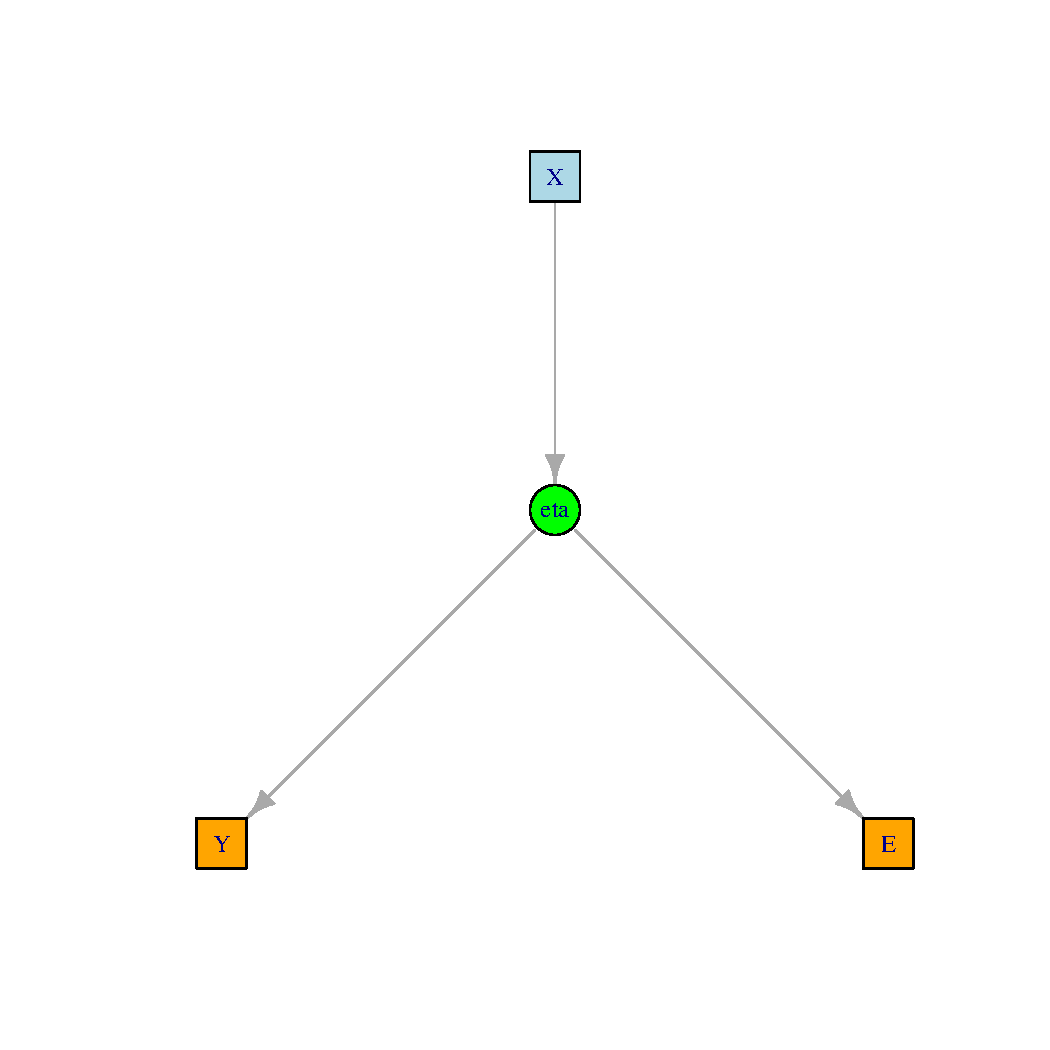
\includegraphics[width=0.5\textwidth]{./figures/show-bivariateLVM-Age.pdf}
\end{center}

\vspace{-1cm}

This model involves 4 variables (3 observed and 1 latent). We can
write the (full)  \textbf{mean vector} and \textbf{variance-covariance matrix} between all the variables:
\begin{align*}
\mu &= \begin{bmatrix} 
\mu_Y \\ \mu_\eta \\ \mu_E \\ \mu_{X} \\
\end{bmatrix} = \begin{bmatrix} 
\Esp[Y] \\ \Esp[\eta] \\ \Esp[E] \\ \Esp[X] \\
\end{bmatrix} 
\\
\Sigma &= \begin{bmatrix} 
\sigma_{Y,Y} & \sigma_{Y,\eta} & \sigma_{Y,E} & \sigma_{Y,X} \\ & \sigma_{\eta,\eta} & \sigma_{\eta,E} & \sigma_{\eta,X} \\ & & \sigma_{E,E} & \sigma_{E,X} \\ &&& \sigma_{X,X}  \\
\end{bmatrix} = \begin{bmatrix} 
\Var(Y) & \Cov(Y,\eta) & \Cov(Y,E) & \Cov(Y,X) \\ & \Var(\eta) & \Cov(\eta,E) & \Cov(\eta,X) \\ & & \Var(E) & \Cov(E,X)  \\ & & & \Var[X]\\
\end{bmatrix} 
\end{align*}
As before we will constrain the mean of the latent variable to be 0
and its variance to be 1. Furthermore, conditional on the latent
variable, \(Y\), \(E\), and \(\eta\) are independent of each other. So
\(\Cov(Y,E)\), \(\Cov(Y,X)\), and \(\Cov(E,X)\) are not "real"
parameters. So we only need to estimate 9 parameters:
\begin{align*}
\theta = \left( \mu_Y, \mu_E, \mu_X, \sigma_{Y,Y}, \sigma_{E,E}, \sigma_{X,X}, \sigma_{Y,\eta}, \sigma_{E,\eta}, \sigma_{\eta,X} \right)
\end{align*}
The \textbf{empirical mean vector} and \textbf{empirical variance-covariance matrix}
also contain 9 parameters:
\begin{align*}
m = \begin{bmatrix} 
\overline{Y} \\ \overline{E} \\ \overline{X} \\
\end{bmatrix} 
\qquad
S = \begin{bmatrix} 
s_{Y,Y} & s_{Y,E} & s_{Y,X} \\ & s_{E,E} & s_{E,X} \\ & & s_{X,X} \\
\end{bmatrix} 
\end{align*}

or in R:
\lstset{language=r,label= ,caption= ,captionpos=b,numbers=none}
\begin{lstlisting}
set.seed(10)
df.2YX <- sim(lvm.2YX, n = 1e4, latent = FALSE)
cbind(mu=colMeans(df.2YX), vcov = cov(df.2YX))
\end{lstlisting}

\begin{verbatim}
           mu         Y          E         X
Y  0.47355535 1.5787540  3.2020009 0.2519949
E  1.17255908 3.2020009 11.5908969 0.7315259
X -0.02028518 0.2519949  0.7315259 0.9781732
\end{verbatim}

So the model satisfy one necessary condition for being
identifiable. This condition is however not sufficient to ensure
identifiability but is easier to check than the NSC (nessary and
sufficient condition). To check the NSC we need to write down the
equations relating the empirical and the theoretical moments. To make
things a little simpler we will assume that \(X\) has mean 0 and
variance 1. We obtain the model:
\begin{align*}
Y &= \mu_Y + \sigma_{Y,\eta} \eta + \varepsilon_Y \qquad \varepsilon_Y\sim\Gaus[0,\sigma_{Y,Y}] \\
E &= \mu_E + \sigma_{E,\eta} \eta + \varepsilon_E \qquad \varepsilon_Y\sim\Gaus[0,\sigma_{E,E}]\\
\eta &= \sigma_{\eta,X} X + \xi_\eta \qquad \varepsilon_\eta\sim\Gaus[0,1]
\end{align*}
we get:
\begin{align*}
\left\{
\begin{array}{l}
s_{Y,Y} = \sigma_{Y,\eta}^2(1+\sigma^2_{\eta,X}) + \sigma_{Y,Y} \\
s_{E,E} = \sigma_{E,\eta}^2(1+\sigma^2_{\eta,X}) + \sigma_{E,E} \\
s_{Y,E} = \sigma_{Y,\eta}\sigma_{E,\eta}(1+\sigma^2_{\eta,X}) \\
s_{Y,X} = \sigma_{Y,\eta}\sigma_{\eta,X} \\
s_{E,X} = \sigma_{E,\eta}\sigma_{\eta,X} 
\end{array}
\right.
\qquad
\left\{
\begin{array}{l}
\sigma_{\eta,X} = \sqrt{\frac{s_{Y,X}s_{E,X}}{s_{Y,E}-s_{Y,X}s_{E,X}}} \\
\sigma_{Y,\eta} = \frac{s_{Y,X}}{\sigma_{\eta,X}} \\
\sigma_{E,\eta} = \frac{s_{E,X}}{\sigma_{\eta,X}} \\
\sigma_{Y,Y} = s_{Y,Y} - \sigma_{Y,\eta}^2(1+\sigma^2_{\eta,X}) \\
\sigma_{E,E} = s_{E,E} - \sigma_{E,\eta}^2(1+\sigma^2_{\eta,X}) \\
\end{array}
\right.
\end{align*}
which we can solve and therefore the model is identifiable. This is
confirmed by the fact that lava is able to estimate the model:
\lstset{language=r,label= ,caption= ,captionpos=b,numbers=none}
\begin{lstlisting}
e.lvm.2XY <- estimate(lvm(Y~eta,E~eta,eta[0:1]~X), data = df.2YX)
e.lvm.2XY
\end{lstlisting}

\begin{verbatim}
                    Estimate Std. Error  Z-value  P-value
Measurements:                                            
   Y~eta             1.01882    0.01931 52.76797   <1e-12
   E~eta             2.95758    0.05605 52.76797   <1e-12
Regressions:                                             
   eta~X             0.25286    0.01119 22.59794   <1e-12
Intercepts:                                              
   Y                 0.47878    0.01231 38.90703   <1e-12
   E                 1.18773    0.03324 35.73453   <1e-12
Residual Variances:                                      
   Y                 0.47569    0.03712 12.81639         
   E                 2.29545    0.30930  7.42139
\end{verbatim}

We can in fact manually estimat the coefficients (here we do REML
estimation instead of ML so the estimated variance will be a bit
larger compared to lava):

\lstset{language=r,label= ,caption= ,captionpos=b,numbers=none}
\begin{lstlisting}
s_YY <- var(df.2YX$Y)
s_EE <- var(df.2YX$E)
s_YX <- cov(df.2YX$Y,df.2YX$X)
s_EX <- cov(df.2YX$E,df.2YX$X)
s_YE <- cov(df.2YX$Y,df.2YX$E)

ratio <- s_EX / (s_YE - s_YX * s_EX)

manual <- c("eta~X" = sqrt(s_YX * ratio),
	    "Y~eta" = s_YX/sqrt(s_YX * ratio),
	    "E~eta" = s_EX/sqrt(s_YX * ratio),
	    "Y~~Y" = s_YY - s_YX^2/(s_YX * ratio) * (1 + s_YX * ratio),
	    "E~~E" =  s_EE - s_EX^2/(s_YX * ratio) * (1 + s_YX * ratio)
	    )
rbind(manual = manual,
      lava = coef(e.lvm.2XY)[names(manual)]
      )
\end{lstlisting}

\begin{verbatim}
           eta~X    Y~eta    E~eta      Y~~Y     E~~E
manual 0.2471585 1.019568 2.959744 0.4757339 2.295681
lava   0.2528586 1.018822 2.957578 0.4756863 2.295452
\end{verbatim}

Note that the model is exactly identifiable in the sense that we have
exactly the same number of parameters and moments. Adding an
additional link between age and one outcome would make the model non
identifiable since we would increase by one the number of parameters
(p=10) while still having only 9 moments:
\lstset{language=r,label= ,caption= ,captionpos=b,numbers=none}
\begin{lstlisting}
estimate(lvm(Y~eta+Age,E~eta,eta[0:1]~X), data = df.2YX)
\end{lstlisting}

\begin{verbatim}
                    Estimate Std. Error  Z-value  P-value
Measurements:                                            
   Y~eta             1.01882    0.01931 52.76797   <1e-12
   E~eta             2.95758    0.05605 52.76797   <1e-12
Regressions:                                             
   eta~X             0.25286    0.01119 22.59794   <1e-12
Intercepts:                                              
   Age               0.47878    0.01231 38.90703   <1e-12
   E                 1.18773    0.03324 35.73453   <1e-12
Residual Variances:                                      
   Y                 0.36434                             
   Age               0.11135                             
   E                 2.29545    0.30930  7.42139         
Warning messages:
1: In sqrt(diag(asVar)) : production de NaN
2: In print.lvmfit(x) : Small singular value: 2.409293e-13
\end{verbatim}
\end{document}